\chapter{Single-atom resolved momentum measurement of lattice Bose gas}

blah blah blah

\section{Metastable Helium}

Metastable Helium, noted $\mathrm{He}^*$, is kind of an odd atom in the ensemble of species that we know how to bring to quantum degeneracy. Its most important feature, which is actually the reason why we chose this atom to measure correlation functions in momentum space, is the existence of the metastable state $2 \ ^3 S_1$. This excited state is called metastable for its very long lifetime of the order of $8,000 \ \mathrm{s}$, far larger than what is required for experiments. Very interestingly, as Helium is a noble gas, the amount of energy required to excite Helium into its metastable state is quite large, $19.8 \ \rm{eV}$. This large energy is sufficient for a metastable Helium atom to extract an electron from an electronic surface. This opens the way for \textbf{electronic detection} techniques, in opposition to the much more widely spread optical detection techniques, that allows for \textbf{single atom detection} as we will see in this chapter. In addition, the energy level structure (see Fig.-\ref{fig:niveaux}) is well adapted to laser cooling with a transition in the near-infrared around $\lambda_0 \simeq 1083 \ \mathrm{nm}$ for which reliable laser sources are available. Metastable Helium was actually amongst the first atoms to be brought to quantum degeneracy with the first BEC of $\He$ being obtained in 2001 simultaneously at the Institut d'Optique and Laboratoire Kastler Brossel in France. Helium also has the advantage to have a stable, albeit very rare and expensive fermionic isotope $^3 \He$ that has also been brought to quantum degeneracy at the Amsterdam LaserLab in 2006.

In spite of all these advantages, $\He$ comes with a few experimental difficulties that explain why they are actually quite few $\He$ experiments over the world. First, Helium is a very light atom and this comes with some very practical difficulties like the need for pre-cooling with liquid nitrogen and quite long Zeeman slowers. Second, $\He$ is subject to Penning collisions that bring back an atom to the ground state to ionize the other:

\begin{equation}
    \He + \He \rightarrow \mathrm{He} + \mathrm{He}^+ + \mathrm{e}^{-}
\end{equation}

Such a reaction thus results in the loss of two atoms and must be avoided. \NOTE{FINIR}

\begin{figure}
    \centering
    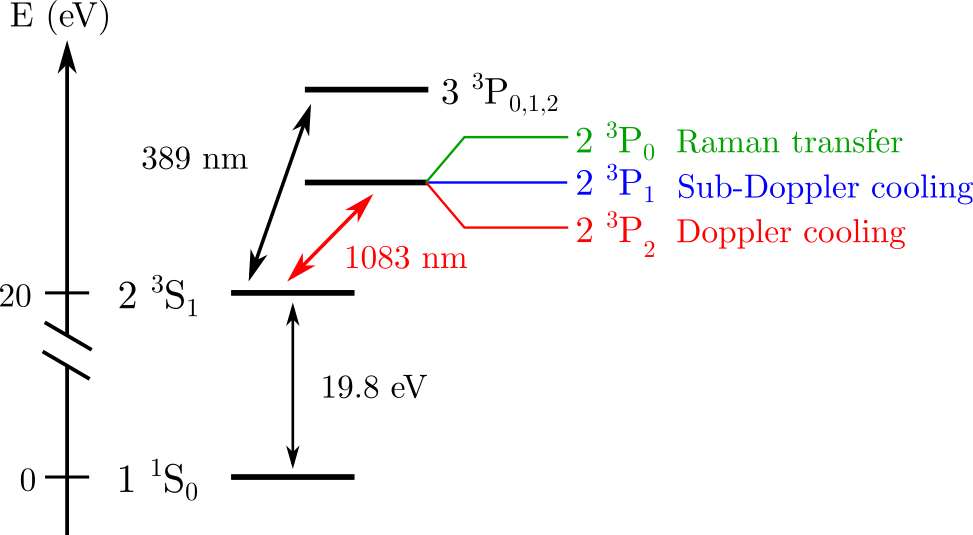
\includegraphics[width=0.9\textwidth]{Fig/Chapter3/niveaux.png}
    \caption{Energy levels of the Helium atom. The metastable state is the triplet state $2 \ ^3S_1$ that we will call the ground state of the metastable Helium atom. Laser cooling is performed on the optical transition $2 \ ^3S_1 \rightarrow 2 \ ^3 P$ of wavelength $\lambda_0 \simeq 1083 \ \mathrm{nm}$. More specifically, we address the transition to  $2 \ ^3 P_2$ or $2 \ ^3 P_1$ depending on the cooling scheme (respectively Doppler and sub-Doppler), as well as the transition to  $2 \ ^3 P_0$ to perform two-photon Raman transfer as we will detail later on.}
    \label{fig:niveaux}
\end{figure}

In the following, we will detail the different experimental steps used to bring a gas of metastable Helium to quantum degeneracy.

\section{Bose-Einstein Condensation of metastable helium}

\subsection{The source}

To begin the experimental sequence, we first need to excite helium atoms in the metastable state. As the energy difference between the ground-state and the metastable state is very large, it is impossible to excite the atoms optically, we therefore rather do it through a plasma discharge. The setup is illustrated on Fig.-\ref{fig:source}. The plasma forms between a metallic needle connected to a high voltage power supply ($\sim 2.8 \ \mathrm{kV}$) and the grounded skimmer. The needle is held in a glass tube that is glued to a \textbf{Boron-Nitride (BN)} piece, in which a small hole is pierced for atoms to flow through. The piece is inserted into a larger copper piece cryogenically cooled with liquid nitrogen. The role of the Boron-Nitride piece is two fold. First, the good thermal properties of the Boron-Nitride allows the piece to be cooled via the contact with the copper, cooling down in turn the atoms. This is necessary to preliminary reduce the speed of the atoms before laser cooling as we will discuss in the next paragraph. Second, the piece isolates the high voltage needle from the grounded copper to avoid plasma formation in unwanted places.

\begin{figure}
    \centering
    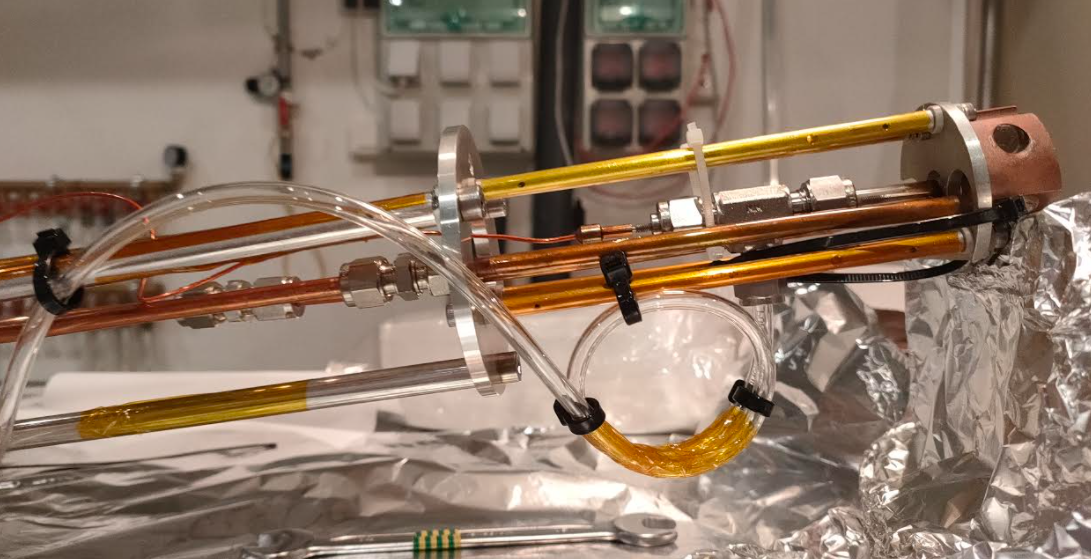
\includegraphics[width=0.9\textwidth]{Fig/Chapter3/source.png}
    \caption{Metastable helium source. a) Illustrative drawing of the source apparatus. Helium atoms (blue arrows) are sent into a glass tube glued into a pierced boron-nitride (BN) piece. A plasma forms between the high voltage needle and the grounded skimmer, exciting the atoms in the metastable state (red arrows). The boron nitride is cooled by thermal contact with a copper (Cu) piece in which liquid nitrogen flows, allowing to significantly reduce the speed of the atoms. b) Photograph of the source apparatus. The red square illustrates what is represented on the drawing.}
    \label{fig:source}
\end{figure}

The source is a quite sensitive part of the experimental apparatus and was often subject to problems during the span of this thesis. Here are a few things that we learned through the different repairs:

\begin{itemize}
    \item The needle has the tendency to deteriorate over time. When this happens, some metallic particles fall from the needle and end up clogging the small hole in Boron-Nitride, preventing the atoms to flow through. We replaced the needle with a standard metallic cylinder, hoping that it would not deteriorate as fast. While we still could form the plasma without the needle shape, the cylinder still deteriorates, requiring regular operations every few months to unclog the Boron-Nitride piece.
    \item The diameter of the Boron-Nitride piece needs to be very well adapted to the inner diameter of the copper piece to ensure a good thermal contact and to prevent the Boron-Nitride from moving when temperature changes.
    \item The glue can contract at low temperatures and add mechanical constraints on the glass tube, sometimes breaking it and causing unwanted atom leakage.
\end{itemize}

Let us now move on the next experimental step, laser cooling.


\subsection{Laser cooling}

Our experimental cooling sequence revolves around two types of laser cooling: Doppler and sub-Doppler cooling. Doppler cooling revolves around the absorption of resonant, counter-propagating photons by a two-level atom, reducing its momentum. The absorbed photons are re-emitted spontaneously in a random direction of space, meaning that after a large number of absorption/emission cycles, the variation of momentum induced by spontaneous emission averages out. The only contribution is thus the one of absorption contributing to slow the atom down. This effect is called Doppler cooling as the frequency of the photons seen by the atoms changes with their speed because of the well-known Doppler effect. It is then necessary to account for the Doppler effect to ensure that the photons are resonant with the two-level transition of interest to ensure proper cooling. On the other hand, sub-Doppler cooling designs a variety of cooling techniques revolving around multi-level atomic structures. These techniques allow to reach lower temperature than Doppler cooling, at the expense of small velocity captures, attainable with prior Doppler cooling. 

As shown on Fig.-\ref{fig:niveaux}, we use the $2 \ ^3 S_1 \rightarrow 2 \ ^3 P_2$ transition for Doppler cooling. The state $2 \ ^3 S_1$ has three sub-states $m_j=\{-1,0,+1\}$ whereas the state $2 \ ^3 P_2$ has 5 $m_j=\{-2,-1,0,+1,+2\}$. By using circularly polarised light allowing transitions that increase or decrease $m_j$ by $1$, the transition between these two-states can be assimilated as an effective two-level transition after a few cycles of absorption/emissions, making it well suited for Doppler cooling. For sub-Doppler cooling, we use the transition  $2 \ ^3 S_1 \rightarrow 2 \ ^3 P_1$ where the excited state also has three sub-states, implementing an effective 3-level lambda structure. The natural line-width of the $2 \ ^3 P$ state is $\Gamma = 2 \pi \times 1.6 \ \rm{MHz}$.

We will not explain here all the details of how laser cooling works, but rather briefly show the main cooling steps of the experimental sequence and give typical experimental numbers. For further details, we refer the reader to previous thesis \cite{hoend2014,bouton_these,cayla_these}.

\NOTE{PARLER DES MELASSES TRANSVERSES ?}

\subsubsection{Zeeman slower}

As in most cold atoms experiment, the cooling sequence starts with a Zeeman slower. The general idea is to exploit the Zeeman effect with a variating magnetic field to compensate the Doppler shift that reduces as the atoms get slower. This procedure allows to reduce the speed of the atoms of several order of magnitudes, from roughly $1,200 \ \rm{m/s}$ when they exit the source to $50 \ \rm{m/s}$, a speed at which they can be captured in a Magneto-Optical Trap. Note that as helium is very light, our Zeeman slower is quite long compared to other cold atom experiments with a length of $\sim 2.5 \ \rm{m}$. This also explains the need for liquid nitrogen cooling of the source, without which we would need an absurdly long Zeeman slower.

\subsubsection{Magneto-Optical Trap}

While reducing the speed of the atoms is necessary to reach quantum degeneracy, it is also necessary to spatially trap the atoms. This is achieved by combining the radiative pressure force with the magnetic force whose role is to trap the atoms. This is the idea behind the \textbf{Magneto-Optical Trap} (MOT), the cornerstone of every cold atom experiment. A MOT is made of 3 pairs of counter-propagating red-detuned laser beams, one for each direction of space, on which we add a quadrupole magnetic field. In our case, the magnetic field is produced by two coils centered on the $x$-axis in anti-Helmoltz configuration. The current is \NOTE{VALUE}, resulting in a gradient of $25 \ \mathrm{G/cm}$ at the center of trap.

To load the MOT, we use an intensity of roughly $15 \ \Isat$ per beam and a strong detuning $\delta =$ \NOTE{VALUE?}. This serves two purposes: it ensures a large capture velocity, making the loading of the trap efficient, and also keeps the level of light-assisted Penning losses low. We load typically \fcolorbox{red}{white}{$N \simeq 2 \times 10^9$} atoms in $\sim 1.5 \ \mathrm{s}$. In a second time, we look to compress the gas to increase the atomic density by reducing the detuning to $\delta =$ \NOTE{VALUE?}. To avoid major Penning losses, we conjointly reduce the total intensity from $90 \ \Isat$ to $0.7 \ \Isat$. This increases the density by a factor 10.

At the end of the MOT phase, we obtain a gas of $N \simeq 2 \times 10^9$ atoms at $T=1.2 \rm{mK}$ of density $n=$\NOTE{VALUE?}.

\subsubsection{Red molasses}

The magnetic field is then switched off to go back to regular Doppler cooling. To further cool the atoms, the detuning is significantly reduced to $\delta=$\NOTE{VALUE?}, while the total intensity is reduced to $0.33 \ \Isat$ to keep the rate of Penning losses constant. The goal is not to reach the lowest possible temperature, but rather to reach a temperature low enough to go under the velocity capture of sub-Doppler cooling effects. After $5 \ \rm{ms}$ of red molasses, we reach $T=120 \ \mu \rm{K}$ with $N\simeq 1.8 \times 10^9$ atoms.

\subsubsection{Gray molasses}

\NOTE{TO DO}

\subsection{Evaporative cooling}

The cooling steps we have described so far are not enough to reach the kinds of temperatures and 

\section{3D optical lattice}

\section{Electronic detection: The Micro Channel Plate Detector}

\section{Two-photon Raman transfer}

\subsection{Principle of the two-photon Raman transfer}

\subsection{Experimental implementation}

\section{Characterisation of two-body collisions in the time-of-flight dynamics}

\subsection{Classical model}

\subsection{Evolution with total atom number}

\subsection{Evolution with lattice depth}

\subsection{Conclusion}

\section{Adabiatic preparation in the vicinity of the Mott transition}

\subsection{Thermometry method}

\subsection{Fischer information and Cramér-Rao bound}

\subsection{Entropy measurement}
